\chapter{Modelo Objeto-Relacional (Ismael)}
\label{ch:ismael}

En este capítulo se implementa el subsistema de \textbf{Publicidad} del sistema EKIS utilizando el modelo Objeto-Relacional de Oracle Database. Este enfoque permite tratar los anuncios no como registros planos, sino como objetos complejos que encapsulan tanto sus datos (título, fechas) como su lógica de negocio (verificación de vigencia) y estructuras anidadas (lista de características del público objetivo).

\section{Instalación y Configuración del Entorno}

Para la realización de esta práctica, se ha optado por desplegar Oracle Database 21c Express Edition (XE) utilizando tecnología de contenedores Docker sobre un sistema operativo Ubuntu Linux. Esta arquitectura permite aislar el SGBD del sistema anfitrión, evitando conflictos de dependencias y facilitando una instalación limpia.

El proceso técnico seguido fue el siguiente:

\begin{enumerate}
    \item \textbf{Despliegue del contenedor:} Se utilizó la imagen \texttt{gvenzl/oracle-xe}, mapeando el puerto 1521 para permitir conexiones externas.
    \item \textbf{Conexión mediante SQL*Plus:} Se accedió a la interfaz de línea de comandos del contenedor para realizar las tareas administrativas.
    \item \textbf{Creación de usuario:} Se creó un usuario específico para la práctica (\texttt{c\#\#ismael}) siguiendo la nomenclatura de usuarios comunes de la arquitectura \textit{multitenant} de Oracle (prefijo \texttt{c\#\#}), otorgándole permisos de conexión y recursos ilimitados.
\end{enumerate}

La siguiente figura muestra la secuencia de comandos utilizada en la terminal para verificar la instalación, conectar al sistema y preparar el usuario de trabajo:

\begin{figure}[H]
    \centering
    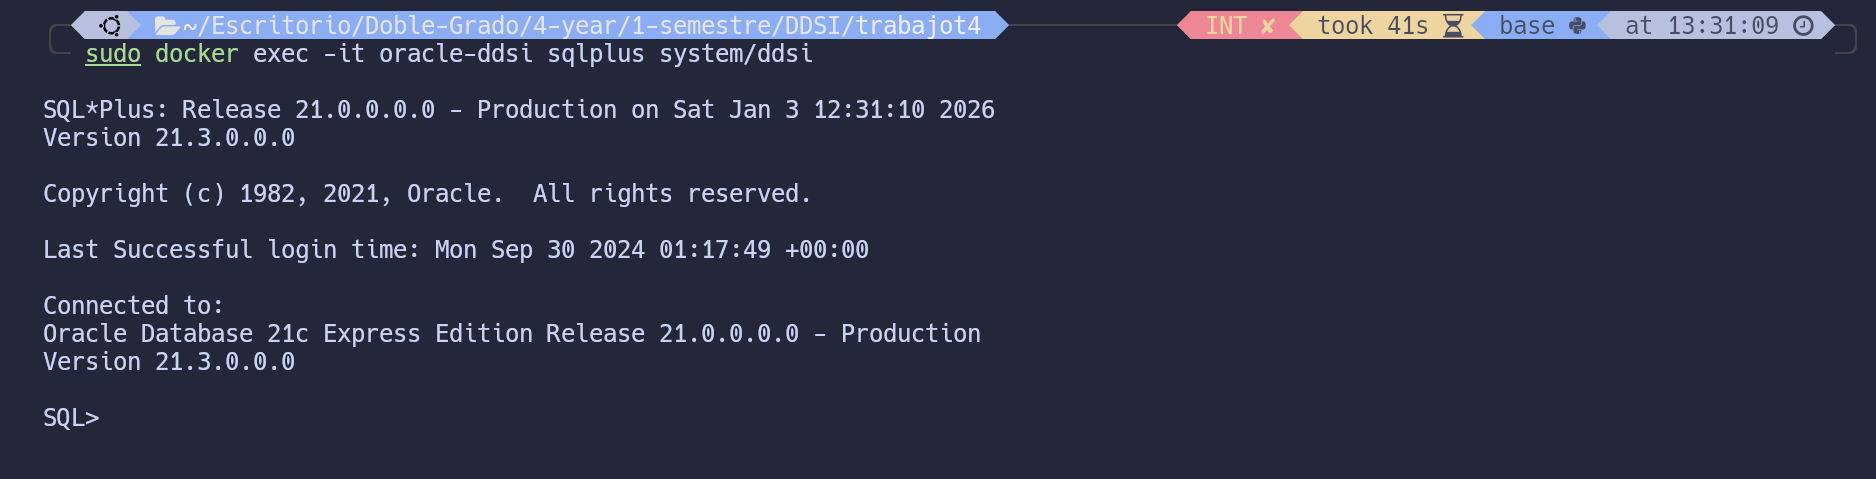
\includegraphics[width=1.0\textwidth]{figures/ismael/instalacion_oracle.png}
    \caption{Secuencia de arranque del contenedor, conexión vía SQL*Plus y creación del usuario c\#\#ismael.}
    \label{fig:oracle_install}
\end{figure}

\section{Diseño Objeto-Relacional del Subsistema}

A diferencia del modelo relacional clásico utilizado en prácticas anteriores, aquí se ha diseñado una estructura jerárquica de tipos para soportar la complejidad de los anuncios de EKIS:

\begin{itemize}
    \item \textbf{Caracteristica\_obj}: Objeto simple que define un criterio de segmentación (ej. Nombre: ''Edad'', Valor: ''18-25'').
    \item \textbf{Lista\_Caracteristicas\_typ}: Un tipo colección (\textit{Nested Table}) que permite almacenar múltiples características dentro de un solo anuncio, eliminando la necesidad de una tabla intermedia de relación N:M típica del modelo relacional puro.
    \item \textbf{Anuncio\_obj}: El objeto principal que encapsula los datos del anuncio y métodos miembros para calcular su estado (activo/caducado) dinámicamente.
\end{itemize}

\section{Implementación DDL y DML}

\subsection{Creación de Tipos y Tablas (DDL)}

Primero, definimos el tipo para el público objetivo y la colección que permitirá el anidamiento:

\begin{minted}{sql}
CREATE OR REPLACE TYPE Caracteristica_obj AS OBJECT (
    nombre_carac VARCHAR2(50),
    valor_carac  VARCHAR2(50),
    MEMBER FUNCTION to_string RETURN VARCHAR2
);
/
CREATE OR REPLACE TYPE Lista_Caracteristicas_typ AS TABLE OF Caracteristica_obj;
\end{minted}

Posteriormente, definimos el objeto \texttt{Anuncio\_obj} que contiene la lógica de negocio mediante el método \texttt{es\_activo}, y creamos la tabla de objetos asociada:

\begin{minted}{sql}
CREATE OR REPLACE TYPE Anuncio_obj AS OBJECT (
    id_anuncio    NUMBER,
    titulo        VARCHAR2(100),
    -- (...) otros atributos (cuerpo, enlace)
    fecha_fin     DATE,
    publico_objetivo Lista_Caracteristicas_typ, -- Atributo complejo (Colección)

    MEMBER FUNCTION es_activo RETURN VARCHAR2,
    MEMBER PROCEDURE mostrar_informacion
);
/
-- Creación de la Tabla de Objetos (Object Table)
CREATE TABLE Tabla_Anuncios OF Anuncio_obj
NESTED TABLE publico_objetivo STORE AS Store_Caracteristicas;
\end{minted}

\subsection{Manipulación de Datos (DML)}

La inserción demuestra la capacidad de instanciar objetos anidados directamente en una sentencia SQL (utilizando constructores), vinculando las características del público objetivo al anuncio en el momento de su creación sin necesidad de múltiples \texttt{INSERT}:

\begin{minted}{sql}
INSERT INTO Tabla_Anuncios VALUES (
    Anuncio_obj(
        101, 'Rebajas Verano EKIS', 'Descuentos ropa',
        TO_DATE('01/01/2026', 'DD/MM/YYYY'),
        TO_DATE('30/01/2026', 'DD/MM/YYYY'),
        -- Instanciación de la colección anidada
        Lista_Caracteristicas_typ(
            Caracteristica_obj('Edad', '18-30'),
            Caracteristica_obj('Ubicacion', 'Granada')
        )
    )
);
\end{minted}

Para la consulta, utilizamos un bloque PL/SQL que recupera el objeto y ejecuta su método \texttt{mostrar\_informacion()}. Esto demuestra cómo el procesamiento de datos se mueve hacia la base de datos:

\begin{minted}{sql}
DECLARE
    v_anuncio Anuncio_obj;
BEGIN
    SELECT VALUE(a) INTO v_anuncio FROM Tabla_Anuncios a WHERE a.id_anuncio = 101;
    -- El método imprime si está ACTIVO o CADUCADO automáticamente
    v_anuncio.mostrar_informacion();
END;
/
\end{minted}

\begin{figure}[H]
    \centering
    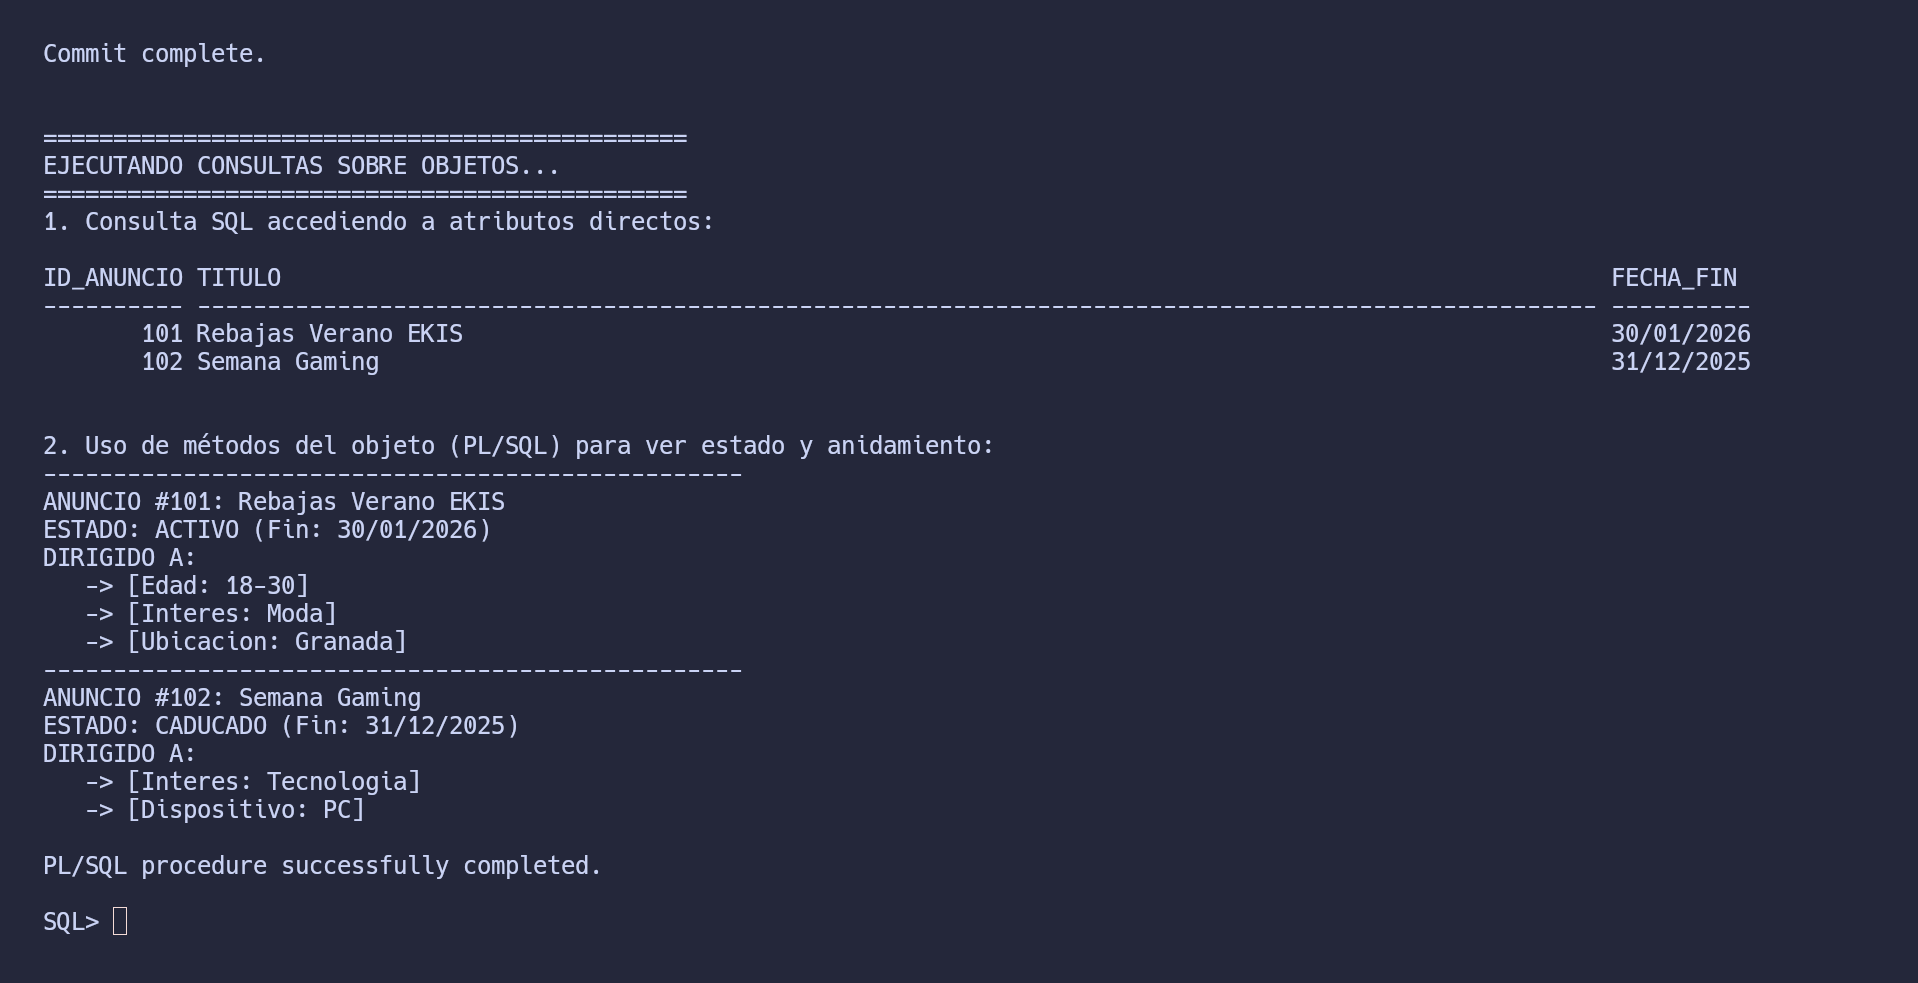
\includegraphics[width=0.9\textwidth]{figures/ismael/consulta_oracle.png}
    \caption{Ejecución de métodos sobre objetos Anuncio y recorrido de tablas anidadas en la terminal.}
    \label{fig:oracle_query}
\end{figure}

\section{Adecuación al Sistema EKIS}

El uso del modelo Objeto-Relacional para el módulo de Publicidad de EKIS presenta ventajas claras frente al relacional puro implementado en la práctica anterior:

\begin{itemize}
    \item \textbf{Encapsulamiento de Lógica:} La lógica para determinar si un anuncio es visible (\texttt{es\_activo}) reside en el propio objeto en la base de datos. Esto garantiza la consistencia, ya que cualquier aplicación que recupere el objeto obtendrá el estado correcto sin reimplementar la lógica de fechas.
    \item \textbf{Simplificación del Modelo:} El uso de \textit{Nested Tables} para el ''Público Objetivo'' elimina la complejidad de gestionar claves foráneas y tablas de unión manualmente para las características, permitiendo tratar el anuncio y sus criterios de segmentación como una unidad atómica lógica.
\end{itemize}